\documentclass[11pt,]{article}
\usepackage[left=1in,top=1in,right=1in,bottom=1in]{geometry}
\newcommand*{\authorfont}{\fontfamily{phv}\selectfont}
\usepackage[]{mathpazo}


  \usepackage[T1]{fontenc}
  \usepackage[utf8]{inputenc}



\usepackage{abstract}
\renewcommand{\abstractname}{}    % clear the title
\renewcommand{\absnamepos}{empty} % originally center

\renewenvironment{abstract}
 {{%
    \setlength{\leftmargin}{0mm}
    \setlength{\rightmargin}{\leftmargin}%
  }%
  \relax}
 {\endlist}

\makeatletter
\def\@maketitle{%
  \newpage
%  \null
%  \vskip 2em%
%  \begin{center}%
  \let \footnote \thanks
    {\fontsize{18}{20}\selectfont\raggedright  \setlength{\parindent}{0pt} \@title \par}%
}
%\fi
\makeatother




\setcounter{secnumdepth}{3}

\usepackage{color}
\usepackage{fancyvrb}
\newcommand{\VerbBar}{|}
\newcommand{\VERB}{\Verb[commandchars=\\\{\}]}
\DefineVerbatimEnvironment{Highlighting}{Verbatim}{commandchars=\\\{\}}
% Add ',fontsize=\small' for more characters per line
\usepackage{framed}
\definecolor{shadecolor}{RGB}{248,248,248}
\newenvironment{Shaded}{\begin{snugshade}}{\end{snugshade}}
\newcommand{\KeywordTok}[1]{\textcolor[rgb]{0.13,0.29,0.53}{\textbf{#1}}}
\newcommand{\DataTypeTok}[1]{\textcolor[rgb]{0.13,0.29,0.53}{#1}}
\newcommand{\DecValTok}[1]{\textcolor[rgb]{0.00,0.00,0.81}{#1}}
\newcommand{\BaseNTok}[1]{\textcolor[rgb]{0.00,0.00,0.81}{#1}}
\newcommand{\FloatTok}[1]{\textcolor[rgb]{0.00,0.00,0.81}{#1}}
\newcommand{\ConstantTok}[1]{\textcolor[rgb]{0.00,0.00,0.00}{#1}}
\newcommand{\CharTok}[1]{\textcolor[rgb]{0.31,0.60,0.02}{#1}}
\newcommand{\SpecialCharTok}[1]{\textcolor[rgb]{0.00,0.00,0.00}{#1}}
\newcommand{\StringTok}[1]{\textcolor[rgb]{0.31,0.60,0.02}{#1}}
\newcommand{\VerbatimStringTok}[1]{\textcolor[rgb]{0.31,0.60,0.02}{#1}}
\newcommand{\SpecialStringTok}[1]{\textcolor[rgb]{0.31,0.60,0.02}{#1}}
\newcommand{\ImportTok}[1]{#1}
\newcommand{\CommentTok}[1]{\textcolor[rgb]{0.56,0.35,0.01}{\textit{#1}}}
\newcommand{\DocumentationTok}[1]{\textcolor[rgb]{0.56,0.35,0.01}{\textbf{\textit{#1}}}}
\newcommand{\AnnotationTok}[1]{\textcolor[rgb]{0.56,0.35,0.01}{\textbf{\textit{#1}}}}
\newcommand{\CommentVarTok}[1]{\textcolor[rgb]{0.56,0.35,0.01}{\textbf{\textit{#1}}}}
\newcommand{\OtherTok}[1]{\textcolor[rgb]{0.56,0.35,0.01}{#1}}
\newcommand{\FunctionTok}[1]{\textcolor[rgb]{0.00,0.00,0.00}{#1}}
\newcommand{\VariableTok}[1]{\textcolor[rgb]{0.00,0.00,0.00}{#1}}
\newcommand{\ControlFlowTok}[1]{\textcolor[rgb]{0.13,0.29,0.53}{\textbf{#1}}}
\newcommand{\OperatorTok}[1]{\textcolor[rgb]{0.81,0.36,0.00}{\textbf{#1}}}
\newcommand{\BuiltInTok}[1]{#1}
\newcommand{\ExtensionTok}[1]{#1}
\newcommand{\PreprocessorTok}[1]{\textcolor[rgb]{0.56,0.35,0.01}{\textit{#1}}}
\newcommand{\AttributeTok}[1]{\textcolor[rgb]{0.77,0.63,0.00}{#1}}
\newcommand{\RegionMarkerTok}[1]{#1}
\newcommand{\InformationTok}[1]{\textcolor[rgb]{0.56,0.35,0.01}{\textbf{\textit{#1}}}}
\newcommand{\WarningTok}[1]{\textcolor[rgb]{0.56,0.35,0.01}{\textbf{\textit{#1}}}}
\newcommand{\AlertTok}[1]{\textcolor[rgb]{0.94,0.16,0.16}{#1}}
\newcommand{\ErrorTok}[1]{\textcolor[rgb]{0.64,0.00,0.00}{\textbf{#1}}}
\newcommand{\NormalTok}[1]{#1}

\usepackage{graphicx,grffile}
\makeatletter
\def\maxwidth{\ifdim\Gin@nat@width>\linewidth\linewidth\else\Gin@nat@width\fi}
\def\maxheight{\ifdim\Gin@nat@height>\textheight\textheight\else\Gin@nat@height\fi}
\makeatother
% Scale images if necessary, so that they will not overflow the page
% margins by default, and it is still possible to overwrite the defaults
% using explicit options in \includegraphics[width, height, ...]{}
\setkeys{Gin}{width=\maxwidth,height=\maxheight,keepaspectratio}

\title{Mi proyecto\\
Vecindad y autocorrelación espacial\\
Proyecto Final de Analis Espacial\\
Profesor :Jose Ramon Martinez Batlle  }



\author{\Large Maria Magdalena Viloria y Adalberto Guerrero P.\vspace{0.05in} \newline\normalsize\emph{Estudiante, Universidad Autónoma de Santo Domingo (UASD)}  }


\date{}

\usepackage{titlesec}

\titleformat*{\section}{\normalsize\bfseries}
\titleformat*{\subsection}{\normalsize\itshape}
\titleformat*{\subsubsection}{\normalsize\itshape}
\titleformat*{\paragraph}{\normalsize\itshape}
\titleformat*{\subparagraph}{\normalsize\itshape}

\titlespacing{\section}
{0pt}{36pt}{0pt}
\titlespacing{\subsection}
{0pt}{36pt}{0pt}
\titlespacing{\subsubsection}
{0pt}{36pt}{0pt}





\newtheorem{hypothesis}{Hypothesis}
\usepackage{setspace}

\makeatletter
\@ifpackageloaded{hyperref}{}{%
\ifxetex
  \PassOptionsToPackage{hyphens}{url}\usepackage[setpagesize=false, % page size defined by xetex
              unicode=false, % unicode breaks when used with xetex
              xetex]{hyperref}
\else
  \PassOptionsToPackage{hyphens}{url}\usepackage[unicode=true]{hyperref}
\fi
}

\@ifpackageloaded{color}{
    \PassOptionsToPackage{usenames,dvipsnames}{color}
}{%
    \usepackage[usenames,dvipsnames]{color}
}
\makeatother
\hypersetup{breaklinks=true,
            bookmarks=true,
            pdfauthor={Maria Magdalena Viloria y Adalberto Guerrero P. (Estudiante, Universidad Autónoma de Santo Domingo (UASD))},
             pdfkeywords = {palabra clave 1, palabra clave 2},  
            pdftitle={Mi proyecto\\
Vecindad y autocorrelación espacial\\
Proyecto Final de Analis Espacial\\
Profesor :Jose Ramon Martinez Batlle},
            colorlinks=true,
            citecolor=blue,
            urlcolor=blue,
            linkcolor=magenta,
            pdfborder={0 0 0}}
\urlstyle{same}  % don't use monospace font for urls

% set default figure placement to htbp
\makeatletter
\def\fps@figure{htbp}
\makeatother

\usepackage{pdflscape} \newcommand{\blandscape}{\begin{landscape}}
\newcommand{\elandscape}{\end{landscape}}


% add tightlist ----------
\providecommand{\tightlist}{%
\setlength{\itemsep}{0pt}\setlength{\parskip}{0pt}}

\begin{document}
	
% \pagenumbering{arabic}% resets `page` counter to 1 
%
% \maketitle

{% \usefont{T1}{pnc}{m}{n}
\setlength{\parindent}{0pt}
\thispagestyle{plain}
{\fontsize{18}{20}\selectfont\raggedright 
\maketitle  % title \par  

}

{
   \vskip 13.5pt\relax \normalsize\fontsize{11}{12} 
\textbf{\authorfont Maria Magdalena Viloria y Adalberto Guerrero P.} \hskip 15pt \emph{\small Estudiante, Universidad Autónoma de Santo Domingo (UASD)}   

}

}








\begin{abstract}

    \hbox{\vrule height .2pt width 39.14pc}

    \vskip 8.5pt % \small 

\noindent Mi resumen


\vskip 8.5pt \noindent \emph{Keywords}: palabra clave 1, palabra clave 2 \par

    \hbox{\vrule height .2pt width 39.14pc}



\end{abstract}


\vskip 6.5pt


\noindent  \section{Introducción}\label{introducciuxf3n}

`A que cree que se debe la delincuencia en el pais ¿A la falta de
alternativas sanas (clubes, cine, teatro, etc.) para el
entretenimiento?: Si'

\section{Metodología}\label{metodologuxeda}

El objetivo de este proyecto es el análisis exploratorio de datos
espaciales, funciones de homogeneidad espacial, tipos de vecindad,
ponderadores y con el índice de autocorrelación espacial de Moran.

Usaremos como referencia la capa de provincias dominicanas y los
resultados de la Encuesta Nacional de Hogares de Propósitos Múltiples de
2017 (ENHOGAR-2017, de. Te usaremos la pregunta de investigacion, sobre
la cual sera realizado el análisis de autocorrelación al final.

\ldots
\#\# Paquetes

\begin{itemize}
\tightlist
\item
  Carga el paquete \texttt{sf}, la colección \texttt{tidyverse} y los
  paquetes \texttt{spdep}, \texttt{lmtest}, \texttt{tmap} y
  \texttt{RColorBrewer}
\end{itemize}

\begin{Shaded}
\begin{Highlighting}[]
\KeywordTok{library}\NormalTok{(sf)}
\end{Highlighting}
\end{Shaded}

\begin{verbatim}
## Linking to GEOS 3.7.1, GDAL 2.4.2, PROJ 5.2.0
\end{verbatim}

\begin{Shaded}
\begin{Highlighting}[]
\KeywordTok{library}\NormalTok{(tidyverse)}
\end{Highlighting}
\end{Shaded}

\begin{verbatim}
## -- Attaching packages --------------------------------------------- tidyverse 1.2.1 --
\end{verbatim}

\begin{verbatim}
## v ggplot2 3.2.1     v purrr   0.3.3
## v tibble  2.1.3     v dplyr   0.8.3
## v tidyr   1.0.0     v stringr 1.4.0
## v readr   1.3.1     v forcats 0.4.0
\end{verbatim}

\begin{verbatim}
## -- Conflicts ------------------------------------------------ tidyverse_conflicts() --
## x dplyr::filter() masks stats::filter()
## x dplyr::lag()    masks stats::lag()
\end{verbatim}

\begin{Shaded}
\begin{Highlighting}[]
\KeywordTok{library}\NormalTok{(spdep)}
\end{Highlighting}
\end{Shaded}

\begin{verbatim}
## Loading required package: sp
\end{verbatim}

\begin{verbatim}
## Loading required package: spData
\end{verbatim}

\begin{verbatim}
## To access larger datasets in this package, install the spDataLarge
## package with: `install.packages('spDataLarge',
## repos='https://nowosad.github.io/drat/', type='source')`
\end{verbatim}

\begin{Shaded}
\begin{Highlighting}[]
\KeywordTok{library}\NormalTok{(lmtest)}
\end{Highlighting}
\end{Shaded}

\begin{verbatim}
## Loading required package: zoo
\end{verbatim}

\begin{verbatim}
## 
## Attaching package: 'zoo'
\end{verbatim}

\begin{verbatim}
## The following objects are masked from 'package:base':
## 
##     as.Date, as.Date.numeric
\end{verbatim}

\begin{Shaded}
\begin{Highlighting}[]
\KeywordTok{library}\NormalTok{(tmap)}
\KeywordTok{library}\NormalTok{(RColorBrewer)}
\end{Highlighting}
\end{Shaded}

\subsection{Datos y unión}\label{datos-y-uniuxf3n}

\begin{itemize}
\tightlist
\item
  Carga el conjunto de datos de ``ENHOGAR 2017'' (\texttt{.csv}),
  asignándolo al objeto \texttt{en17}. Nota que ``ENHOGAR 2017'' es una
  encuesta y, por lo tanto, recoge resultados referidos a una muestra,
  cuyo tamaño por provincia está recogido en la columna
  \texttt{muestra}. Carga también la capa geométrica (\texttt{.gpkg})
  asignándola al objeto \texttt{prov}, y únelo a \texttt{en17}. Ambas
  fuentes se encuentran en la carpeta \texttt{data}. Recuerda el
  problema de la inconsistencia en el código entre ambas fuentes.
  Verifica consistencia luego de corregir el código (usa la práctica
  anterior como apoyo). Finalmente, une ambas fuentes, \texttt{prov} y
  \texttt{en17}.
\end{itemize}

\begin{Shaded}
\begin{Highlighting}[]
\NormalTok{en17 <-}\StringTok{ }\KeywordTok{read.csv}\NormalTok{(}\StringTok{'material-de-apoyo-master/data/enhogar_2017.csv'}\NormalTok{, }\DataTypeTok{check.names =}\NormalTok{ F)}
\NormalTok{prov <-}\StringTok{ }\KeywordTok{st_read}\NormalTok{(}\DataTypeTok{dsn =} \StringTok{'material-de-apoyo-master/data/divisionRD.gpkg'}\NormalTok{, }\DataTypeTok{layer =} \StringTok{'PROVcenso2010'}\NormalTok{)}
\end{Highlighting}
\end{Shaded}

\begin{verbatim}
## Reading layer `PROVcenso2010' from data source `/home/franc/unidad-0-asignacion-99-mi-proyecto-Adalbertogp2020/material-de-apoyo-master/data/divisionRD.gpkg' using driver `GPKG'
## Simple feature collection with 32 features and 4 fields
## geometry type:  MULTIPOLYGON
## dimension:      XY
## bbox:           xmin: 182215.8 ymin: 1933532 xmax: 571365.3 ymax: 2205216
## epsg (SRID):    32619
## proj4string:    +proj=utm +zone=19 +datum=WGS84 +units=m +no_defs
\end{verbatim}

\begin{Shaded}
\begin{Highlighting}[]
\NormalTok{en17 <-}\StringTok{ }\NormalTok{en17 }\OperatorTok\StringTok{ }\KeywordTok{mutate}\NormalTok{(}\DataTypeTok{ENLACE =} \KeywordTok{ifelse}\NormalTok{(}\KeywordTok{nchar}\NormalTok{(Código)}\OperatorTok{==}\DecValTok{3}\NormalTok{, }\KeywordTok{paste0}\NormalTok{(}\StringTok{'0'}\NormalTok{, Código),Código))}
\KeywordTok{match}\NormalTok{(en17}\OperatorTok{$}\NormalTok{ENLACE, prov}\OperatorTok{$}\NormalTok{ENLACE)}
\end{Highlighting}
\end{Shaded}

\begin{verbatim}
##  [1]  9 18 25 13 24 28  6 14 19 20  5 15 26 27  2 17 21 31  3  4 10 16  7
## [24] 22  8 11 12 23 29 30  1 32
\end{verbatim}

\begin{Shaded}
\begin{Highlighting}[]
\NormalTok{proven17 <-}\StringTok{ }\NormalTok{prov }\OperatorTok\StringTok{ }\KeywordTok{inner_join}\NormalTok{(en17, }\DataTypeTok{by =} \StringTok{'ENLACE'}\NormalTok{)}
\end{Highlighting}
\end{Shaded}

\begin{verbatim}
## Warning: Column `ENLACE` joining factor and character vector, coercing into
## character vector
\end{verbatim}

\begin{itemize}
\tightlist
\item
  Se Imprime en pantalla el \texttt{sf} resultante y genera un mapa que
  muestre tu pregunta para todo el país.
\end{itemize}

\begin{Shaded}
\begin{Highlighting}[]
\NormalTok{proven17 }\OperatorTok
\StringTok{  }\NormalTok{dplyr}\OperatorTok{::}\KeywordTok{select}\NormalTok{(}\KeywordTok{contains}\NormalTok{(}\StringTok{'A que cree que se debe la delincuencia en el pais ¿A la falta de alternativas sanas (clubes, cine, teatro, etc.) para el entretenimiento?: Si'}\NormalTok{)) }\OperatorTok
\StringTok{  }\KeywordTok{plot}\NormalTok{(}\DataTypeTok{breaks =} \StringTok{'jenks'}\NormalTok{)}
\end{Highlighting}
\end{Shaded}

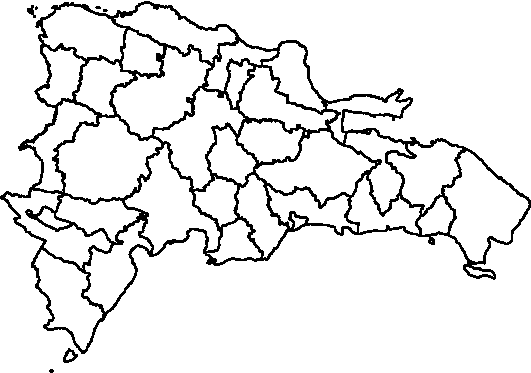
\includegraphics{proyecto_files/figure-latex/unnamed-chunk-3-1.pdf}

\subsection{\texorpdfstring{Conversión a
\texttt{sp}}{Conversión a sp}}\label{conversiuxf3n-a-sp}

\begin{itemize}
\tightlist
\item
  Conviertiendo el objeto \texttt{proven17} a
  \texttt{SpatialPolygonsDataFrame} asignándolo a \texttt{proven17.sp},
  mediante la función \texttt{as\_Spatial}. Este paso es necesario para
  crear los objetos de vecindad. Verificamos que los nombres de columnas
  \texttt{proven17.sp} aparecen deformados (espacios sustituidos por
  puntos), y lo corrígimos rescatando los nombres del objeto original
  \texttt{proven17}.
\end{itemize}

\begin{Shaded}
\begin{Highlighting}[]
\NormalTok{proven17.sp <-}\StringTok{ }\KeywordTok{as_Spatial}\NormalTok{(proven17)}
\KeywordTok{colnames}\NormalTok{(proven17.sp}\OperatorTok{@}\NormalTok{data)[}\DecValTok{1}\OperatorTok{:}\DecValTok{20}\NormalTok{]}
\end{Highlighting}
\end{Shaded}

\begin{verbatim}
##  [1] "PROV"                                                                               
##  [2] "REG"                                                                                
##  [3] "TOPONIMIA"                                                                          
##  [4] "ENLACE"                                                                             
##  [5] "Código"                                                                             
##  [6] "Provincia"                                                                          
##  [7] "Principales.problemas.de.su.barrio.o.comunidad...La.falta.de.energía.eléctrica...Si"
##  [8] "Principales.problemas.de.su.barrio.o.comunidad...La.falta.de.energía.eléctrica...No"
##  [9] "Principales.problemas.de.su.barrio.o.comunidad...La.delincuencia...Si"              
## [10] "Principales.problemas.de.su.barrio.o.comunidad...La.delincuencia...No"              
## [11] "Principales.problemas.de.su.barrio.o.comunidad...El.desempleo...Si"                 
## [12] "Principales.problemas.de.su.barrio.o.comunidad...El.desempleo...No"                 
## [13] "Principales.problemas.de.su.barrio.o.comunidad...La.pobreza...Si"                   
## [14] "Principales.problemas.de.su.barrio.o.comunidad...La.pobreza...No"                   
## [15] "Principales.problemas.de.su.barrio.o.comunidad...El.consumo.de.drogas...Si"         
## [16] "Principales.problemas.de.su.barrio.o.comunidad...El.consumo.de.drogas...No"         
## [17] "Principales.problemas.de.su.barrio.o.comunidad...La.venta.de.drogas...Si"           
## [18] "Principales.problemas.de.su.barrio.o.comunidad...La.venta.de.drogas...No"           
## [19] "Principales.problemas.de.su.barrio.o.comunidad...El.costo.de.la.vida...Si"          
## [20] "Principales.problemas.de.su.barrio.o.comunidad...El.costo.de.la.vida...No"
\end{verbatim}

\begin{Shaded}
\begin{Highlighting}[]
\KeywordTok{colnames}\NormalTok{(proven17.sp}\OperatorTok{@}\NormalTok{data) <-}\StringTok{ }\NormalTok{proven17 }\OperatorTok\StringTok{ }\KeywordTok{st_drop_geometry}\NormalTok{() }\OperatorTok\StringTok{ }\NormalTok{colnames}
\end{Highlighting}
\end{Shaded}

\begin{itemize}
\tightlist
\item
  Asignamos nombres de filas al objeto \texttt{proven17.sp} a partir de
  la columna \texttt{TOPONIMIA}.
\end{itemize}

\begin{Shaded}
\begin{Highlighting}[]
\KeywordTok{row.names}\NormalTok{(proven17.sp) <-}\StringTok{ }\KeywordTok{as.character}\NormalTok{(proven17.sp}\OperatorTok{$}\NormalTok{TOPONIMIA)}
\end{Highlighting}
\end{Shaded}

\subsection{Vecindad por contigüidad}\label{vecindad-por-contiguxfcidad}

\begin{itemize}
\tightlist
\item
  A partir de \texttt{proven17.sp}, creamos un objeto de vecindad por
  contigüidad, asignándolo a \texttt{proven17.nb}, usando criterio
  \texttt{queen}. Se Imprime en pantalla el resumen de dicho objeto de
  vecindad.
\end{itemize}

\begin{Shaded}
\begin{Highlighting}[]
\NormalTok{proven17.nb <-}\StringTok{ }\KeywordTok{poly2nb}\NormalTok{(proven17.sp, }\DataTypeTok{queen=}\OtherTok{TRUE}\NormalTok{)}
\KeywordTok{summary}\NormalTok{(proven17.nb)}
\end{Highlighting}
\end{Shaded}

\begin{verbatim}
## Neighbour list object:
## Number of regions: 32 
## Number of nonzero links: 144 
## Percentage nonzero weights: 14.0625 
## Average number of links: 4.5 
## Link number distribution:
## 
##  1  2  3  4  5  6  7  8  9 
##  1  2  5 11  5  4  2  1  1 
## 1 least connected region:
## DISTRITO NACIONAL with 1 link
## 1 most connected region:
## LA VEGA with 9 links
\end{verbatim}

\begin{itemize}
\tightlist
\item
  Evalúamos la cardinalidad, es decir, cuántos vecinos tiene cada
  geometría/elemento (que en este caso son provincias).
\end{itemize}

\begin{Shaded}
\begin{Highlighting}[]
\KeywordTok{card}\NormalTok{(proven17.nb)}
\end{Highlighting}
\end{Shaded}

\begin{verbatim}
##  [1] 1 6 4 4 3 7 4 4 6 5 2 3 9 3 4 2 3 4 3 4 5 7 5 4 6 6 4 5 8 4 5 4
\end{verbatim}

\begin{itemize}
\tightlist
\item
  Imprimimos en pantalla la relación de vecinos de cada geometría.
\end{itemize}

\begin{Shaded}
\begin{Highlighting}[]
\KeywordTok{sapply}\NormalTok{(proven17.nb, }\ControlFlowTok{function}\NormalTok{(x) x)}
\end{Highlighting}
\end{Shaded}

\begin{verbatim}
## [[1]]
## [1] 32
## 
## [[2]]
## [1]  3  4 13 17 22 31
## 
## [[3]]
## [1]  2  4 10 22
## 
## [[4]]
## [1]  2  3 10 16
## 
## [[5]]
## [1]  7 15 26
## 
## [[6]]
## [1]  9 13 14 19 20 24 29
## 
## [[7]]
## [1]  5 10 22 26
## 
## [[8]]
## [1] 11 12 23 30
## 
## [[9]]
## [1]  6 13 14 18 19 25
## 
## [[10]]
## [1]  3  4  7 16 22
## 
## [[11]]
## [1]  8 12
## 
## [[12]]
## [1]  8 11 23
## 
## [[13]]
## [1]  2  6  9 19 22 24 25 28 31
## 
## [[14]]
## [1]  6  9 20
## 
## [[15]]
## [1]  5 18 26 27
## 
## [[16]]
## [1]  4 10
## 
## [[17]]
## [1]  2 21 31
## 
## [[18]]
## [1]  9 15 25 27
## 
## [[19]]
## [1]  6  9 13
## 
## [[20]]
## [1]  6 14 29 30
## 
## [[21]]
## [1] 17 28 29 31 32
## 
## [[22]]
## [1]  2  3  7 10 13 25 26
## 
## [[23]]
## [1]  8 12 29 30 32
## 
## [[24]]
## [1]  6 13 28 29
## 
## [[25]]
## [1]  9 13 18 22 26 27
## 
## [[26]]
## [1]  5  7 15 22 25 27
## 
## [[27]]
## [1] 15 18 25 26
## 
## [[28]]
## [1] 13 21 24 29 31
## 
## [[29]]
## [1]  6 20 21 23 24 28 30 32
## 
## [[30]]
## [1]  8 20 23 29
## 
## [[31]]
## [1]  2 13 17 21 28
## 
## [[32]]
## [1]  1 21 23 29
\end{verbatim}

\begin{itemize}
\tightlist
\item
  Construimos un mapa de los vínculos de vecindad (grafo). Recuerdar que
  primero debemos de generar un mapa de las provincias, y luego se
  superpondrán los vínculos.
\end{itemize}

\begin{Shaded}
\begin{Highlighting}[]
\KeywordTok{plot}\NormalTok{(proven17.sp, }\DataTypeTok{border=}\StringTok{"grey"}\NormalTok{, }\DataTypeTok{lwd=}\FloatTok{0.5}\NormalTok{)}
\KeywordTok{plot}\NormalTok{(proven17.nb, }\KeywordTok{coordinates}\NormalTok{(proven17.sp), }\DataTypeTok{add=}\NormalTok{T)}
\end{Highlighting}
\end{Shaded}

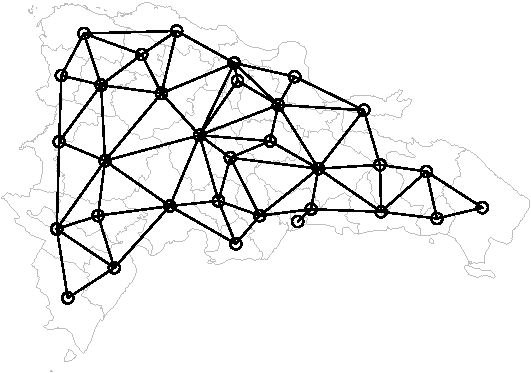
\includegraphics{proyecto_files/figure-latex/unnamed-chunk-9-1.pdf} *
Evalúamos si el objeto de vecindad es simétrico.

\begin{Shaded}
\begin{Highlighting}[]
\KeywordTok{is.symmetric.nb}\NormalTok{(proven17.nb)}
\end{Highlighting}
\end{Shaded}

\begin{verbatim}
## [1] TRUE
\end{verbatim}

\subsection{Vecindad por número de
vecinos}\label{vecindad-por-nuxfamero-de-vecinos}

\begin{itemize}
\tightlist
\item
  A partir de \texttt{proven17.sp}, crearemos un objeto de vecindad por
  número de vecinos, en el que cada geometría tenga sólo un vecino,
  asignándolo a \texttt{proven17.nb.k1}. Imprime en pantalla el resumen
  de dicho objeto de vecindad. Recuerda crear un objeto de coordenadas
  de centroides, que en este ejercicio se sugiere con el nombre
  \texttt{coords}, y otro de identidades de cada geometría, para el cual
  se sugiere el nombre \texttt{ident}; ambos los usarás dentro de la
  función \texttt{knn2nb} El resumen del objeto \texttt{proven17.nb.k1}
  debería mostrar 32 vínculos, el mismo número de regiones de
  \texttt{proven17.sp}, dado que cada región tiene un único vínculo.
\end{itemize}

\begin{Shaded}
\begin{Highlighting}[]
\NormalTok{coords <-}\StringTok{ }\KeywordTok{coordinates}\NormalTok{(proven17.sp)}
\NormalTok{ident <-}\StringTok{ }\KeywordTok{row.names}\NormalTok{(proven17.sp)}
\NormalTok{proven17.nb.k1 <-}\StringTok{ }\KeywordTok{knn2nb}\NormalTok{(}\KeywordTok{knearneigh}\NormalTok{(coords, }\DataTypeTok{k =} \DecValTok{1}\NormalTok{), }\DataTypeTok{row.names =}\NormalTok{ ident)}
\KeywordTok{summary}\NormalTok{(proven17.nb.k1)}
\end{Highlighting}
\end{Shaded}

\begin{verbatim}
## Neighbour list object:
## Number of regions: 32 
## Number of nonzero links: 32 
## Percentage nonzero weights: 3.125 
## Average number of links: 1 
## Non-symmetric neighbours list
## Link number distribution:
## 
##  1 
## 32 
## 32 least connected regions:
## DISTRITO NACIONAL AZUA BAORUCO BARAHONA DAJABÓN DUARTE ELÍAS PIÑA EL SEIBO ESPAILLAT INDEPENDENCIA LA ALTAGRACIA LA ROMANA LA VEGA MARÍA TRINIDAD SÁNCHEZ MONTE CRISTI PEDERNALES PERAVIA PUERTO PLATA HERMANAS MIRABAL SAMANÁ SAN CRISTÓBAL SAN JUAN SAN PEDRO DE MACORÍS SANCHEZ RAMÍREZ SANTIAGO SANTIAGO RODRÍGUEZ VALVERDE MONSEÑOR NOUEL MONTE PLATA HATO MAYOR SAN JOSÉ DE OCOA SANTO DOMINGO with 1 link
## 32 most connected regions:
## DISTRITO NACIONAL AZUA BAORUCO BARAHONA DAJABÓN DUARTE ELÍAS PIÑA EL SEIBO ESPAILLAT INDEPENDENCIA LA ALTAGRACIA LA ROMANA LA VEGA MARÍA TRINIDAD SÁNCHEZ MONTE CRISTI PEDERNALES PERAVIA PUERTO PLATA HERMANAS MIRABAL SAMANÁ SAN CRISTÓBAL SAN JUAN SAN PEDRO DE MACORÍS SANCHEZ RAMÍREZ SANTIAGO SANTIAGO RODRÍGUEZ VALVERDE MONSEÑOR NOUEL MONTE PLATA HATO MAYOR SAN JOSÉ DE OCOA SANTO DOMINGO with 1 link
\end{verbatim}

\begin{itemize}
\tightlist
\item
  Evalúamos la cardinalidad, es decir, cuántos vecinos tiene cada
  geometría/elemento (que en este caso son provincias). Dado que se
  especificó anteriormente que sólo hubiese un único vecino, el vector
  debería ser una repetición de \texttt{1}.
\end{itemize}

\begin{Shaded}
\begin{Highlighting}[]
\KeywordTok{card}\NormalTok{(proven17.nb)}
\end{Highlighting}
\end{Shaded}

\begin{verbatim}
##  [1] 1 6 4 4 3 7 4 4 6 5 2 3 9 3 4 2 3 4 3 4 5 7 5 4 6 6 4 5 8 4 5 4
\end{verbatim}

\begin{itemize}
\tightlist
\item
  Imprime en pantalla la relación de vecinos de cada geometría.
\end{itemize}

\begin{Shaded}
\begin{Highlighting}[]
\KeywordTok{sapply}\NormalTok{(proven17.nb, }\ControlFlowTok{function}\NormalTok{(x) x)}
\end{Highlighting}
\end{Shaded}

\begin{verbatim}
## [[1]]
## [1] 32
## 
## [[2]]
## [1]  3  4 13 17 22 31
## 
## [[3]]
## [1]  2  4 10 22
## 
## [[4]]
## [1]  2  3 10 16
## 
## [[5]]
## [1]  7 15 26
## 
## [[6]]
## [1]  9 13 14 19 20 24 29
## 
## [[7]]
## [1]  5 10 22 26
## 
## [[8]]
## [1] 11 12 23 30
## 
## [[9]]
## [1]  6 13 14 18 19 25
## 
## [[10]]
## [1]  3  4  7 16 22
## 
## [[11]]
## [1]  8 12
## 
## [[12]]
## [1]  8 11 23
## 
## [[13]]
## [1]  2  6  9 19 22 24 25 28 31
## 
## [[14]]
## [1]  6  9 20
## 
## [[15]]
## [1]  5 18 26 27
## 
## [[16]]
## [1]  4 10
## 
## [[17]]
## [1]  2 21 31
## 
## [[18]]
## [1]  9 15 25 27
## 
## [[19]]
## [1]  6  9 13
## 
## [[20]]
## [1]  6 14 29 30
## 
## [[21]]
## [1] 17 28 29 31 32
## 
## [[22]]
## [1]  2  3  7 10 13 25 26
## 
## [[23]]
## [1]  8 12 29 30 32
## 
## [[24]]
## [1]  6 13 28 29
## 
## [[25]]
## [1]  9 13 18 22 26 27
## 
## [[26]]
## [1]  5  7 15 22 25 27
## 
## [[27]]
## [1] 15 18 25 26
## 
## [[28]]
## [1] 13 21 24 29 31
## 
## [[29]]
## [1]  6 20 21 23 24 28 30 32
## 
## [[30]]
## [1]  8 20 23 29
## 
## [[31]]
## [1]  2 13 17 21 28
## 
## [[32]]
## [1]  1 21 23 29
\end{verbatim}

\begin{itemize}
\tightlist
\item
  Hacemos un mapa de los vínculos de vecindad (grafo). Recuerdar que
  primero debemos generar un mapa de las provincias (primera corrida de
  la función \texttt{plot}), y luego le superpondrás el mapa de los
  vínculos (segunda corrida de \texttt{plot}, con argumento
  \texttt{add=T})
\end{itemize}

\begin{Shaded}
\begin{Highlighting}[]
\KeywordTok{plot}\NormalTok{(proven17.sp, }\DataTypeTok{border=}\StringTok{"grey"}\NormalTok{, }\DataTypeTok{lwd=}\FloatTok{0.5}\NormalTok{)}
\KeywordTok{plot}\NormalTok{(proven17.nb.k1, }\KeywordTok{coordinates}\NormalTok{(proven17.sp), }\DataTypeTok{add=}\NormalTok{T)}
\end{Highlighting}
\end{Shaded}

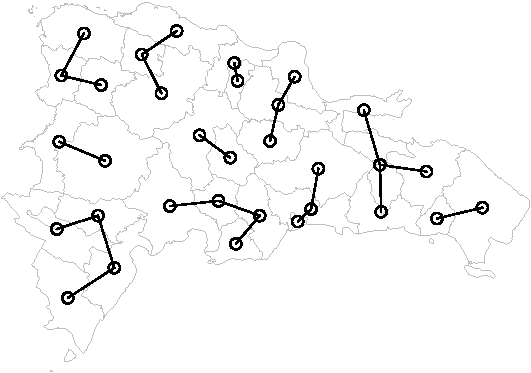
\includegraphics{proyecto_files/figure-latex/unnamed-chunk-14-1.pdf}

\begin{itemize}
\tightlist
\item
  Evalúamos si el objeto de vecindad es simétrico
\end{itemize}

\begin{Shaded}
\begin{Highlighting}[]
\KeywordTok{is.symmetric.nb}\NormalTok{(proven17.nb)}
\end{Highlighting}
\end{Shaded}

\begin{verbatim}
## [1] TRUE
\end{verbatim}

\begin{itemize}
\tightlist
\item
  Exploramos las distancias entre centroides de las geometrías a partir
  del objeto \texttt{proven17.nb.k1}. Para ello, creamos un objeto
  denominado \texttt{dist} donde se almacenan las distancias a partir de
  aplicar la función \texttt{nbdists} (recuerda que dentro de ésta
  debemos colocar el objeto \texttt{coords}). Esto Imprime en pantalla
  un resumen estadístico, y genera un histograma y un boxplot.
\end{itemize}

\begin{Shaded}
\begin{Highlighting}[]
\NormalTok{dist <-}\StringTok{ }\KeywordTok{unlist}\NormalTok{(}\KeywordTok{nbdists}\NormalTok{(proven17.nb.k1, coords))}
\KeywordTok{summary}\NormalTok{(dist)}
\end{Highlighting}
\end{Shaded}

\begin{verbatim}
##    Min. 1st Qu.  Median    Mean 3rd Qu.    Max. 
##   13343   27259   31411   29957   34552   41826
\end{verbatim}

\begin{Shaded}
\begin{Highlighting}[]
\KeywordTok{hist}\NormalTok{(dist)}
\end{Highlighting}
\end{Shaded}

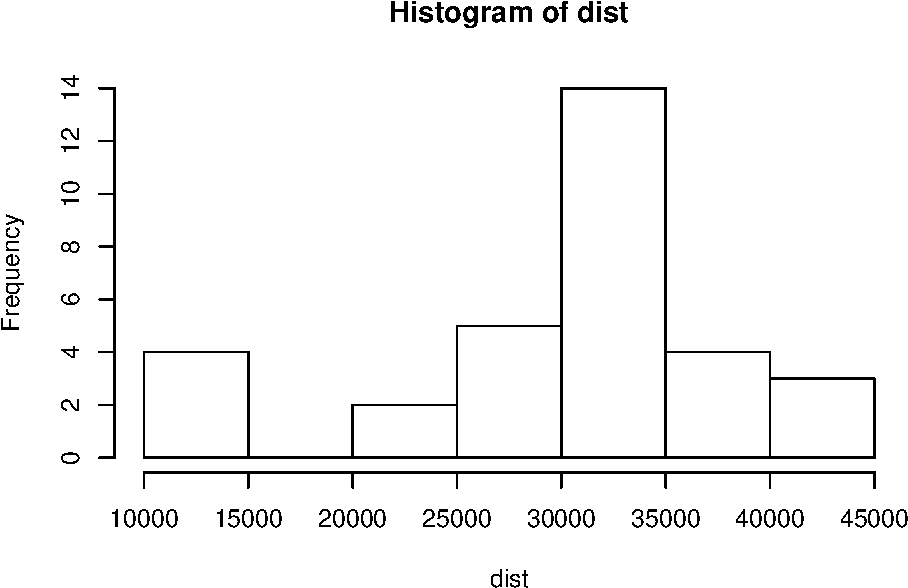
\includegraphics{proyecto_files/figure-latex/unnamed-chunk-16-1.pdf}

\begin{Shaded}
\begin{Highlighting}[]
\KeywordTok{boxplot}\NormalTok{(dist)}
\end{Highlighting}
\end{Shaded}

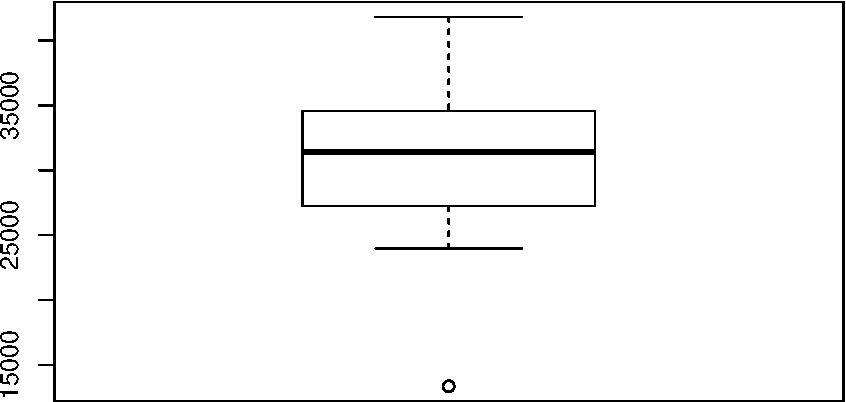
\includegraphics{proyecto_files/figure-latex/unnamed-chunk-16-2.pdf} *
Generaremos un objeto con la distancia mínima (objeto \texttt{distmin}
usando la función \texttt{min}) y otro con la máxima (objeto
\texttt{distmax} usando la función \texttt{max}). Luego, se determina
qué posición ocupa en el vector \texttt{dist} ocupan los valores de
\texttt{distmin} de \texttt{distmax}, y asígnalas a los objetos
\texttt{indicemin} y \texttt{indicemax}, respectivamente.
Posteriormente, utiliza dichas posiciones (\texttt{indicemin} y
\texttt{indicemax}) dentro del índice de \texttt{ident} para determinar
cuál o cuáles provincias se encuentran a la menor y a la mayor distancia
en el conjunto del país.

\begin{Shaded}
\begin{Highlighting}[]
\NormalTok{(distmin <-}\StringTok{ }\KeywordTok{min}\NormalTok{(dist)) }
\end{Highlighting}
\end{Shaded}

\begin{verbatim}
## [1] 13343.28
\end{verbatim}

\begin{Shaded}
\begin{Highlighting}[]
\NormalTok{(distmax <-}\StringTok{ }\KeywordTok{max}\NormalTok{(dist))}
\end{Highlighting}
\end{Shaded}

\begin{verbatim}
## [1] 41826.21
\end{verbatim}

\begin{Shaded}
\begin{Highlighting}[]
\NormalTok{indicemin <-}\StringTok{ }\KeywordTok{which}\NormalTok{(dist}\OperatorTok{==}\NormalTok{distmin)}
\NormalTok{ident[indicemin]}
\end{Highlighting}
\end{Shaded}

\begin{verbatim}
## [1] "DISTRITO NACIONAL" "SANTO DOMINGO"
\end{verbatim}

\begin{Shaded}
\begin{Highlighting}[]
\NormalTok{indicemax <-}\StringTok{ }\KeywordTok{which}\NormalTok{(dist}\OperatorTok{==}\NormalTok{distmax)}
\NormalTok{ident[indicemax]}
\end{Highlighting}
\end{Shaded}

\begin{verbatim}
## [1] "SAMANÁ"
\end{verbatim}

\begin{itemize}
\tightlist
\item
  Ordenaremos los nombres de provincias de menor a mayor distancia de
  separación con su vecino más próximo.
\end{itemize}

\begin{Shaded}
\begin{Highlighting}[]
\NormalTok{ident[}\KeywordTok{order}\NormalTok{(dist)]}
\end{Highlighting}
\end{Shaded}

\begin{verbatim}
##  [1] "DISTRITO NACIONAL"      "SANTO DOMINGO"         
##  [3] "ESPAILLAT"              "HERMANAS MIRABAL"      
##  [5] "DUARTE"                 "MARÍA TRINIDAD SÁNCHEZ"
##  [7] "PERAVIA"                "SAN CRISTÓBAL"         
##  [9] "SANCHEZ RAMÍREZ"        "LA VEGA"               
## [11] "MONSEÑOR NOUEL"         "DAJABÓN"               
## [13] "SANTIAGO RODRÍGUEZ"     "MONTE PLATA"           
## [15] "PUERTO PLATA"           "VALVERDE"              
## [17] "BAORUCO"                "INDEPENDENCIA"         
## [19] "SANTIAGO"               "SAN JOSÉ DE OCOA"      
## [21] "LA ALTAGRACIA"          "LA ROMANA"             
## [23] "EL SEIBO"               "HATO MAYOR"            
## [25] "SAN PEDRO DE MACORÍS"   "MONTE CRISTI"          
## [27] "AZUA"                   "ELÍAS PIÑA"            
## [29] "SAN JUAN"               "BARAHONA"              
## [31] "PEDERNALES"             "SAMANÁ"
\end{verbatim}

\subsection{Ponderadores espaciales}\label{ponderadores-espaciales}

\begin{itemize}
\tightlist
\item
  Generamos dos objetos de pesos espaciales a partir del objeto de
  vecindad por contigüidad; uno de ellos estandarizado por filas
  (asígnalo a \texttt{proven17.w.W}) y otro binario (asígnalo a
  \texttt{proven17.w.B})
\end{itemize}

\begin{Shaded}
\begin{Highlighting}[]
\NormalTok{proven17.w.W <-}\StringTok{ }\KeywordTok{nb2listw}\NormalTok{(proven17.nb)}
\NormalTok{proven17.w.W}
\end{Highlighting}
\end{Shaded}

\begin{verbatim}
## Characteristics of weights list object:
## Neighbour list object:
## Number of regions: 32 
## Number of nonzero links: 144 
## Percentage nonzero weights: 14.0625 
## Average number of links: 4.5 
## 
## Weights style: W 
## Weights constants summary:
##    n   nn S0       S1       S2
## W 32 1024 32 15.83669 132.7525
\end{verbatim}

\begin{Shaded}
\begin{Highlighting}[]
\NormalTok{proven17.w.B <-}\StringTok{ }\KeywordTok{nb2listw}\NormalTok{(proven17.nb, }\DataTypeTok{style =} \StringTok{'B'}\NormalTok{)}
\NormalTok{proven17.w.B}
\end{Highlighting}
\end{Shaded}

\begin{verbatim}
## Characteristics of weights list object:
## Neighbour list object:
## Number of regions: 32 
## Number of nonzero links: 144 
## Percentage nonzero weights: 14.0625 
## Average number of links: 4.5 
## 
## Weights style: B 
## Weights constants summary:
##    n   nn  S0  S1   S2
## B 32 1024 144 288 2968
\end{verbatim}

\subsection{Autocorrelación espacial de nuestra
variable}\label{autocorrelaciuxf3n-espacial-de-nuestra-variable}

Exploramos la autocorrelación espacial de nuestra variable utilizando el
\emph{I} de Moran global y el local.

\begin{itemize}
\tightlist
\item
  Usando \texttt{tidyverse}, generamos una columna de porcentaje de
  personas que respondió a nuestra pregunta respecto del tamaño de la
  muestra a nivel provincial (columna \texttt{muestra}). le Pondremos
  por nombre \texttt{mivariable\_pct}. Generamos una transformada a
  partir de la anterior, y le pondremos el nombre
  \texttt{mivariable\_pct\_log}. El objeto \texttt{sf} resultante se
  asígnara a \texttt{proven17\_mivar\_sf}
\end{itemize}

\begin{Shaded}
\begin{Highlighting}[]
\NormalTok{mivariable <-}\StringTok{ 'A qué cree que se debe la delincuencia en el país: ¿A la falta de alternativas sanas (clubes, cine, teatro, etc.) para el entretenimiento?: Si'}
\NormalTok{proven17_mivar <-}\StringTok{ }\NormalTok{proven17 }\OperatorTok
\StringTok{  }\KeywordTok{st_centroid}\NormalTok{() }\OperatorTok\StringTok{ }
\StringTok{  }\KeywordTok{select}\NormalTok{(ENLACE, }\DataTypeTok{mivariable=}\KeywordTok{contains}\NormalTok{(mivariable), muestra) }\OperatorTok\StringTok{ }
\StringTok{  }\KeywordTok{mutate}\NormalTok{(}\StringTok{'mivariable_pct'}\NormalTok{ =}\StringTok{ }\NormalTok{mivariable}\OperatorTok{/}\NormalTok{muestra}\OperatorTok{*}\DecValTok{100}\NormalTok{,}
         \StringTok{'mivariable_pct_log'}\NormalTok{ =}\StringTok{ }\KeywordTok{log1p}\NormalTok{(mivariable}\OperatorTok{/}\NormalTok{muestra}\OperatorTok{*}\DecValTok{100}\NormalTok{),}
         \DataTypeTok{x=}\KeywordTok{unlist}\NormalTok{(}\KeywordTok{map}\NormalTok{(geom,}\DecValTok{1}\NormalTok{)),}
         \DataTypeTok{y=}\KeywordTok{unlist}\NormalTok{(}\KeywordTok{map}\NormalTok{(geom,}\DecValTok{2}\NormalTok{))) }\OperatorTok
\StringTok{  }\KeywordTok{select}\NormalTok{(}\OperatorTok{-}\NormalTok{muestra) }\OperatorTok\StringTok{ }
\StringTok{  }\KeywordTok{st_drop_geometry}\NormalTok{()}
\end{Highlighting}
\end{Shaded}

\begin{verbatim}
## Warning in st_centroid.sf(.): st_centroid assumes attributes are constant
## over geometries of x
\end{verbatim}

\begin{Shaded}
\begin{Highlighting}[]
\NormalTok{proven17_mivar_sf <-}\StringTok{ }\NormalTok{proven17 }\OperatorTok
\StringTok{  }\KeywordTok{inner_join}\NormalTok{(proven17_mivar, }\DataTypeTok{by =} \StringTok{'ENLACE'}\NormalTok{) }\OperatorTok\StringTok{ }
\StringTok{  }\NormalTok{dplyr}\OperatorTok{::}\KeywordTok{select}\NormalTok{(muestra, }\KeywordTok{contains}\NormalTok{(}\StringTok{'mivariable'}\NormalTok{), x, y, ENLACE, TOPONIMIA)}
\end{Highlighting}
\end{Shaded}

\begin{itemize}
\tightlist
\item
  Hacemos un mapa que muestre la variable, tanto en su versión original
  como transformada.
\end{itemize}

\begin{Shaded}
\begin{Highlighting}[]
\NormalTok{p1 <-}\StringTok{ }\KeywordTok{tm_shape}\NormalTok{(proven17_mivar_sf) }\OperatorTok{+}
\StringTok{  }\KeywordTok{tm_fill}\NormalTok{(}\DataTypeTok{col =} \StringTok{"mivariable_pct"}\NormalTok{, }\DataTypeTok{style =} \StringTok{'jenks'}\NormalTok{,}
          \DataTypeTok{palette =} \KeywordTok{brewer.pal}\NormalTok{(}\DecValTok{9}\NormalTok{, }\DataTypeTok{name =} \StringTok{'Reds'}\NormalTok{), }\DataTypeTok{title =}\NormalTok{ mivariable) }\OperatorTok{+}
\StringTok{  }\KeywordTok{tm_borders}\NormalTok{(}\DataTypeTok{lwd =} \FloatTok{0.5}\NormalTok{)}
\NormalTok{p2 <-}\StringTok{ }\KeywordTok{tm_shape}\NormalTok{(proven17_mivar_sf) }\OperatorTok{+}
\StringTok{  }\KeywordTok{tm_fill}\NormalTok{(}\DataTypeTok{col =} \StringTok{"mivariable_pct_log"}\NormalTok{, }\DataTypeTok{style =} \StringTok{'jenks'}\NormalTok{,}
          \DataTypeTok{palette =} \KeywordTok{brewer.pal}\NormalTok{(}\DecValTok{9}\NormalTok{, }\DataTypeTok{name =} \StringTok{'Reds'}\NormalTok{), }\DataTypeTok{midpoint =} \OtherTok{NA}\NormalTok{, }\DataTypeTok{title =}\NormalTok{ mivariable) }\OperatorTok{+}
\StringTok{  }\KeywordTok{tm_borders}\NormalTok{(}\DataTypeTok{lwd =} \FloatTok{0.5}\NormalTok{) }
\KeywordTok{tmap_arrange}\NormalTok{(p1, p2)}
\end{Highlighting}
\end{Shaded}

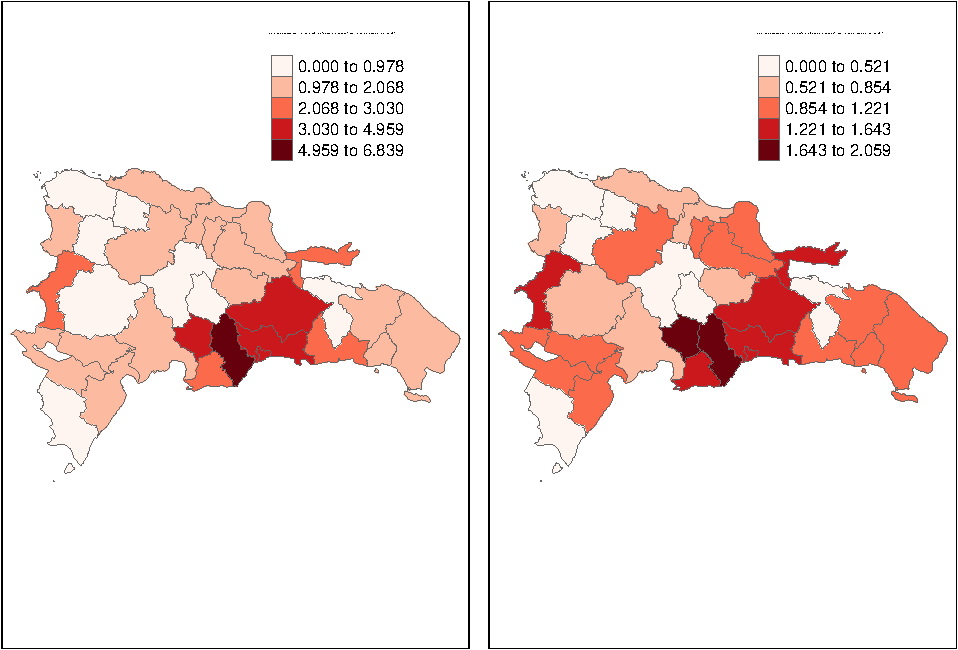
\includegraphics{proyecto_files/figure-latex/pctfueramaps-1.pdf} *
Compruebamos el supuesto de normalidad de nuestra variable, tanto en su
versión original como transformada, mediante el gráfico cuantilar normal
y la prueba de \emph{Shapiro-Wilk}.

\begin{quote}
Tip: Como argumento de las funciones a continuación, usa la forma
vectorial de tu variable original y transformada;
e.g.proven17\_mivar\_sf\$mivariable\_pct\_log
\end{quote}

\begin{quote}
Tip: Si los puntos del gráfico cuantilar normal siguen una línea recta,
y la prueba de Shapiro-Wilk resulta no significativa (es decir, el valor
de \emph{p} mayor que 0.05), entonces se asume como válido el supuesto
de normalidad.
\end{quote}

\begin{Shaded}
\begin{Highlighting}[]
\KeywordTok{qqnorm}\NormalTok{(proven17_mivar_sf}\OperatorTok{$}\NormalTok{mivariable_pct) }\CommentTok{#Versión original de la variable}
\end{Highlighting}
\end{Shaded}

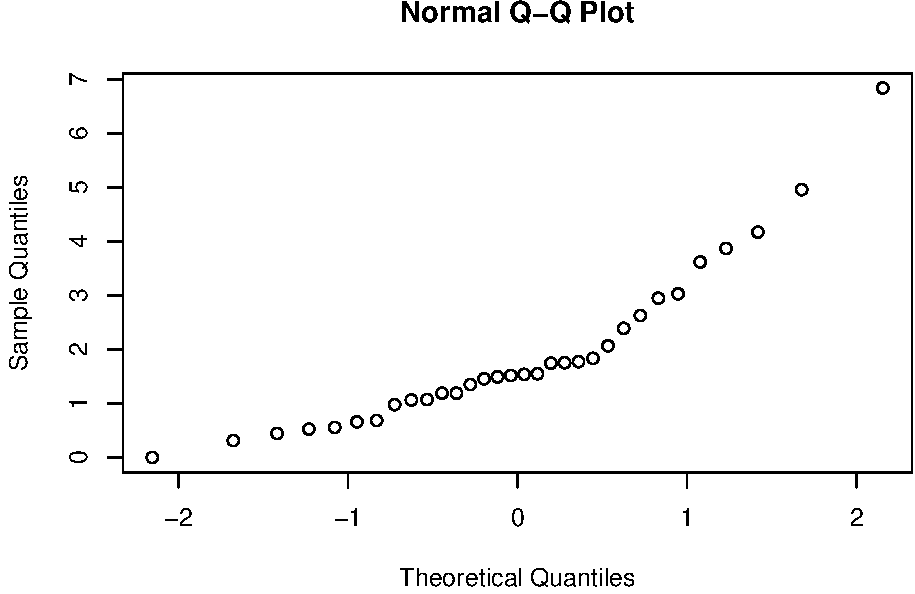
\includegraphics{proyecto_files/figure-latex/unnamed-chunk-21-1.pdf}

\begin{Shaded}
\begin{Highlighting}[]
\KeywordTok{shapiro.test}\NormalTok{(proven17_mivar_sf}\OperatorTok{$}\NormalTok{mivariable_pct) }\CommentTok{#Versión original de la variable}
\end{Highlighting}
\end{Shaded}

\begin{verbatim}
## 
##  Shapiro-Wilk normality test
## 
## data:  proven17_mivar_sf$mivariable_pct
## W = 0.86785, p-value = 0.001036
\end{verbatim}

\begin{Shaded}
\begin{Highlighting}[]
\KeywordTok{qqnorm}\NormalTok{(proven17_mivar_sf}\OperatorTok{$}\NormalTok{mivariable_pct_log) }\CommentTok{#Versión transformada de la variable (log)}
\end{Highlighting}
\end{Shaded}

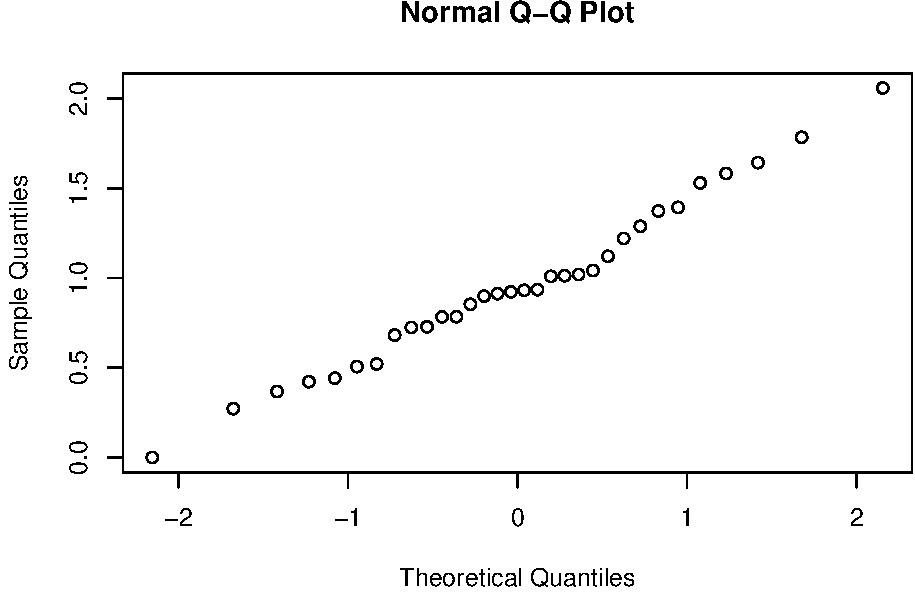
\includegraphics{proyecto_files/figure-latex/unnamed-chunk-21-2.pdf}

\begin{Shaded}
\begin{Highlighting}[]
\KeywordTok{shapiro.test}\NormalTok{(proven17_mivar_sf}\OperatorTok{$}\NormalTok{mivariable_pct_log) }\CommentTok{#Versión transformada de la variable (log)}
\end{Highlighting}
\end{Shaded}

\begin{verbatim}
## 
##  Shapiro-Wilk normality test
## 
## data:  proven17_mivar_sf$mivariable_pct_log
## W = 0.98533, p-value = 0.9311
\end{verbatim}

\section{Resultados}\label{resultados}

\begin{itemize}
\tightlist
\item
  Interpreta el resultado de la comprobación anterior aquí:
\end{itemize}

\section{\texorpdfstring{1-para la variable original=prueba de
Shapiro-Wilk resulta significativa (es decir, el valor de \emph{p} menor
que 0.05), entonces se asume como no válido el supuesto de
normalidad.}{1-para la variable original=prueba de Shapiro-Wilk resulta significativa (es decir, el valor de p menor que 0.05), entonces se asume como no válido el supuesto de normalidad.}}\label{para-la-variable-originalprueba-de-shapiro-wilk-resulta-significativa-es-decir-el-valor-de-p-menor-que-0.05-entonces-se-asume-como-no-vuxe1lido-el-supuesto-de-normalidad.}

\section{\texorpdfstring{2-para la variable modificada=prueba de
Shaprio-Wilk resulta no significativa (es decir, el valor de
\emph{p}mayor que 0.05), entonces se asume como válido el supuesto de
normalidad.}{2-para la variable modificada=prueba de Shaprio-Wilk resulta no significativa (es decir, el valor de pmayor que 0.05), entonces se asume como válido el supuesto de normalidad.}}\label{para-la-variable-modificadaprueba-de-shaprio-wilk-resulta-no-significativa-es-decir-el-valor-de-pmayor-que-0.05-entonces-se-asume-como-vuxe1lido-el-supuesto-de-normalidad.}

\begin{itemize}
\tightlist
\item
  Comprobamos el supuesto de homocedasticidad de tu variable respecto de
  \texttt{x} e \texttt{y}, tanto en su versión original como en la
  transformada, mediante la prueba de \emph{Breusch-Pagan}.
\end{itemize}

\begin{quote}
Tip: Si el valor de \emph{p} es menor que 0.05 (nivel de significancia
convencional, aunque arbitrario), existe evidencia para rechazar la
hipótesis de homocedasticidad.
\end{quote}

\begin{Shaded}
\begin{Highlighting}[]
\NormalTok{proven17_mivar_sf }\OperatorTok\StringTok{ }\KeywordTok{lm}\NormalTok{(mivariable_pct }\OperatorTok{~}\StringTok{ }\NormalTok{x, .) }\OperatorTok\StringTok{ }\KeywordTok{bptest}\NormalTok{()}
\end{Highlighting}
\end{Shaded}

\begin{verbatim}
## 
##  studentized Breusch-Pagan test
## 
## data:  .
## BP = 0.26322, df = 1, p-value = 0.6079
\end{verbatim}

\begin{Shaded}
\begin{Highlighting}[]
\NormalTok{proven17_mivar_sf }\OperatorTok\StringTok{ }\KeywordTok{lm}\NormalTok{(mivariable_pct }\OperatorTok{~}\StringTok{ }\NormalTok{y, .) }\OperatorTok\StringTok{ }\KeywordTok{bptest}\NormalTok{()}
\end{Highlighting}
\end{Shaded}

\begin{verbatim}
## 
##  studentized Breusch-Pagan test
## 
## data:  .
## BP = 3.8733, df = 1, p-value = 0.04906
\end{verbatim}

\begin{Shaded}
\begin{Highlighting}[]
\NormalTok{proven17_mivar_sf }\OperatorTok\StringTok{ }\KeywordTok{lm}\NormalTok{(mivariable_pct_log }\OperatorTok{~}\StringTok{ }\NormalTok{x, .) }\OperatorTok\StringTok{ }\KeywordTok{bptest}\NormalTok{()}
\end{Highlighting}
\end{Shaded}

\begin{verbatim}
## 
##  studentized Breusch-Pagan test
## 
## data:  .
## BP = 0.0025367, df = 1, p-value = 0.9598
\end{verbatim}

\begin{Shaded}
\begin{Highlighting}[]
\NormalTok{proven17_mivar_sf }\OperatorTok\StringTok{ }\KeywordTok{lm}\NormalTok{(mivariable_pct_log }\OperatorTok{~}\StringTok{ }\NormalTok{y, .) }\OperatorTok\StringTok{ }\KeywordTok{bptest}\NormalTok{()}
\end{Highlighting}
\end{Shaded}

\begin{verbatim}
## 
##  studentized Breusch-Pagan test
## 
## data:  .
## BP = 5.4309, df = 1, p-value = 0.01978
\end{verbatim}

\begin{itemize}
\tightlist
\item
  Interpreta el resultado de la comprobación anterior aquí: \#1-para la
  variable original=el valor de \emph{p} es mayor que 0.05 (nivel de
  significancia no convencional, aunque arbitrario), no existe evidencia
  para rechazar la hipótesis de homocedasticidad. \#2-para la variable
  modificada=el valor de \emph{p} es mayor que 0.05 (nivel de
  significancia no convencional, aunque arbitrario), no existe evidencia
  para rechazar la hipótesis de homocedasticidad.
\end{itemize}

En la eventualidad de que el supuesto normalidad y el de
homocedasticidad no se cumplan, continúa con el procedimiento de estimar
la autocorrelación la versión original o la transformada de tu variable,
según elijas, aun cuando los resultados del análisis de autocorrelación
espacial podrían no ser fiables.

\section{Autocorrelación espacial
global}\label{autocorrelaciuxf3n-espacial-global}

\begin{itemize}
\tightlist
\item
  Comprobamos primero que existe consistencia en la secuencia de los
  nombres del objeto de vecindad y el \emph{sf}.
\end{itemize}

\begin{Shaded}
\begin{Highlighting}[]
\KeywordTok{match}\NormalTok{(}\KeywordTok{attr}\NormalTok{(proven17.w.W}\OperatorTok{$}\NormalTok{neighbours, }\StringTok{"region.id"}\NormalTok{), proven17_mivar_sf}\OperatorTok{$}\NormalTok{TOPONIMIA)}\OperatorTok{==}\DecValTok{1}\OperatorTok{:}\DecValTok{32}
\end{Highlighting}
\end{Shaded}

\begin{verbatim}
##  [1] TRUE TRUE TRUE TRUE TRUE TRUE TRUE TRUE TRUE TRUE TRUE TRUE TRUE TRUE
## [15] TRUE TRUE TRUE TRUE TRUE TRUE TRUE TRUE TRUE TRUE TRUE TRUE TRUE TRUE
## [29] TRUE TRUE TRUE TRUE
\end{verbatim}

\begin{itemize}
\tightlist
\item
  Aplicamos la prueba de autocorrelación espacial global para el
  \emph{I} de Moran, usando los pesos estandarizados por filas como los
  binarios.
\end{itemize}

\begin{Shaded}
\begin{Highlighting}[]
\NormalTok{(gmoranw <-}\StringTok{ }\KeywordTok{moran.test}\NormalTok{(}\DataTypeTok{x =}\NormalTok{ proven17_mivar_sf}\OperatorTok{$}\NormalTok{mivariable_pct_log, }\DataTypeTok{listw =}\NormalTok{ proven17.w.W))}
\end{Highlighting}
\end{Shaded}

\begin{verbatim}
## 
##  Moran I test under randomisation
## 
## data:  proven17_mivar_sf$mivariable_pct_log  
## weights: proven17.w.W    
## 
## Moran I statistic standard deviate = 2.2906, p-value = 0.01099
## alternative hypothesis: greater
## sample estimates:
## Moran I statistic       Expectation          Variance 
##        0.23185848       -0.03225806        0.01329463
\end{verbatim}

\begin{Shaded}
\begin{Highlighting}[]
\NormalTok{(gmoranb <-}\StringTok{ }\KeywordTok{moran.test}\NormalTok{(}\DataTypeTok{x =}\NormalTok{ proven17_mivar_sf}\OperatorTok{$}\NormalTok{mivariable_pct_log, }\DataTypeTok{listw =}\NormalTok{ proven17.w.B))}
\end{Highlighting}
\end{Shaded}

\begin{verbatim}
## 
##  Moran I test under randomisation
## 
## data:  proven17_mivar_sf$mivariable_pct_log  
## weights: proven17.w.B    
## 
## Moran I statistic standard deviate = 2.119, p-value = 0.01705
## alternative hypothesis: greater
## sample estimates:
## Moran I statistic       Expectation          Variance 
##        0.19297774       -0.03225806        0.01129866
\end{verbatim}

\begin{itemize}
\tightlist
\item
  Interpreta el resultado de la comprobación anterior aquí:
\end{itemize}

\section{\texorpdfstring{1-para los pesos estandarizados=el valor de
\emph{p} obtenido fue menor de 0.05, hay evidencia preliminar para
rechazar la hipótesis nula de ``no hay autocorrelación espacial'', y por
lo tanto concluir que ``si hay autocorrelación
espacial''}{1-para los pesos estandarizados=el valor de p obtenido fue menor de 0.05, hay evidencia preliminar para rechazar la hipótesis nula de no hay autocorrelación espacial, y por lo tanto concluir que si hay autocorrelación espacial}}\label{para-los-pesos-estandarizadosel-valor-de-p-obtenido-fue-menor-de-0.05-hay-evidencia-preliminar-para-rechazar-la-hipuxf3tesis-nula-de-no-hay-autocorrelaciuxf3n-espacial-y-por-lo-tanto-concluir-que-si-hay-autocorrelaciuxf3n-espacial}

\section{\texorpdfstring{2-para los pesos binarios=el valor de \emph{p}
obtenido fue menor de 0.05, hay evidencia preliminar para rechazar la
hipótesis nula de ``no hay autocorrelación espacial'', y por lo tanto
concluir que ``si hay autocorrelación
espacial''}{2-para los pesos binarios=el valor de p obtenido fue menor de 0.05, hay evidencia preliminar para rechazar la hipótesis nula de no hay autocorrelación espacial, y por lo tanto concluir que si hay autocorrelación espacial}}\label{para-los-pesos-binariosel-valor-de-p-obtenido-fue-menor-de-0.05-hay-evidencia-preliminar-para-rechazar-la-hipuxf3tesis-nula-de-no-hay-autocorrelaciuxf3n-espacial-y-por-lo-tanto-concluir-que-si-hay-autocorrelaciuxf3n-espacial}

\begin{quote}
Tip: Si el valor de \emph{p} obtenido fue menor de 0.05, hay evidencia
preliminar para rechazar la hipótesis nula de ``no hay autocorrelación
espacial'', y por lo tanto concluir que ``sí hay autocorrelación
espacial''. En cualquier caso, es necesario que continúes evaluando la
autocorrelación a nivel local en el siguiente paso, con independencia
del resultado obtenido en la prueba global.
\end{quote}

\begin{itemize}
\tightlist
\item
  Evalúamos la autocorrelación espacial local. Realizamos el diagrama de
  dispersión de Moran (\emph{Moran scatterplot}), mediante la función
  \texttt{moran.plot}. Posteriormente, cargamos el script
  \texttt{lisaclusters.R}, y ejecutamos la función \texttt{lisamap} a
  nuestros datos para generar el mapa LISA. En la función
  \texttt{lisamap}, debemos introducir los siguientes argumentos:
  \texttt{objesp}, que es el objeto espacial denominado
  \texttt{proven17\_mivar\_sf}; \texttt{pesos}, que es el objeto de
  pesos, que será \texttt{proven17.w.W}.
\end{itemize}

\begin{Shaded}
\begin{Highlighting}[]
\KeywordTok{moran.plot}\NormalTok{(}\DataTypeTok{x =}\NormalTok{ proven17_mivar_sf}\OperatorTok{$}\NormalTok{mivariable_pct_log, }\DataTypeTok{listw =}\NormalTok{ proven17.w.W)}
\end{Highlighting}
\end{Shaded}

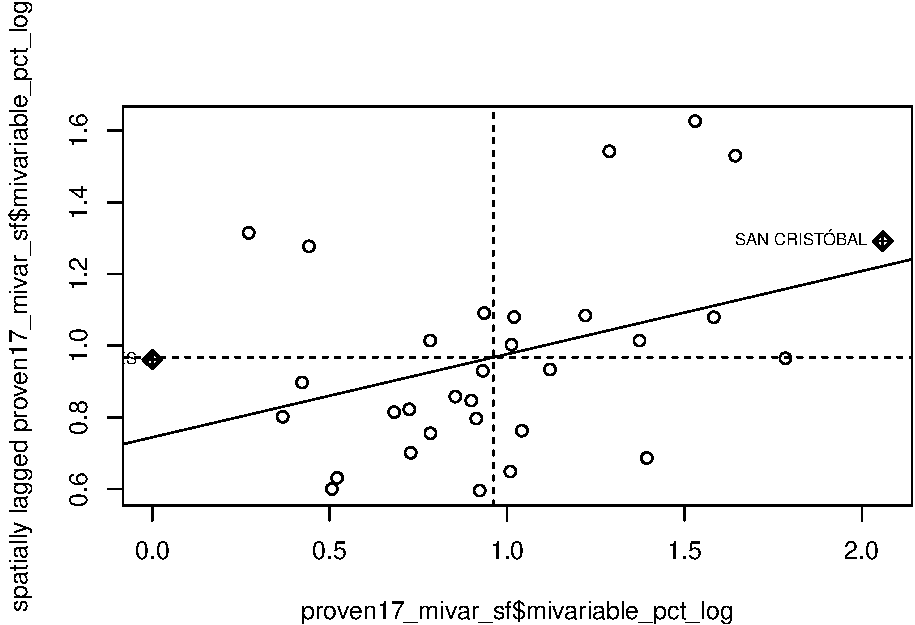
\includegraphics{proyecto_files/figure-latex/unnamed-chunk-25-1.pdf}

\begin{Shaded}
\begin{Highlighting}[]
\KeywordTok{source}\NormalTok{(}\StringTok{'lisaclusters.R'}\NormalTok{)}
\KeywordTok{lisamap}\NormalTok{(}\DataTypeTok{objesp =}\NormalTok{ proven17_mivar_sf,}
        \DataTypeTok{var =} \StringTok{'mivariable_pct_log'}\NormalTok{,}
        \DataTypeTok{pesos =}\NormalTok{ proven17.w.W,}
        \DataTypeTok{tituloleyenda =} \StringTok{'Significancia}\CharTok{\textbackslash{}n}\StringTok{("x-y", léase}\CharTok{\textbackslash{}n}\StringTok{como "x"}\CharTok{\textbackslash{}n}\StringTok{rodeado de "y"'}\NormalTok{,}
        \DataTypeTok{leyenda =}\NormalTok{ T,}
        \DataTypeTok{anchuratitulo =} \DecValTok{1000}\NormalTok{,}
        \DataTypeTok{tamanotitulo =} \DecValTok{16}\NormalTok{,}
        \DataTypeTok{fuentedatos =} \StringTok{'ENHOGAR 2017'}\NormalTok{,}
        \DataTypeTok{titulomapa =} \KeywordTok{paste0}\NormalTok{(}\StringTok{'Clusters LISA de respuestas a la pregunta:}\CharTok{\textbackslash{}n}\StringTok{"'}\NormalTok{, mivariable, }\StringTok{'"'}\NormalTok{))}
\end{Highlighting}
\end{Shaded}

\begin{verbatim}
## $grafico
\end{verbatim}

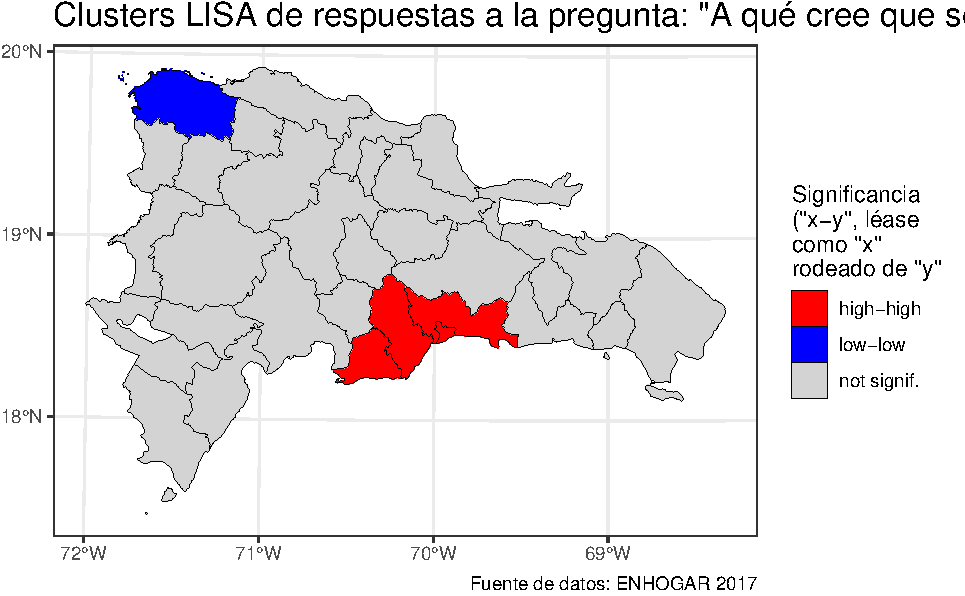
\includegraphics{proyecto_files/figure-latex/unnamed-chunk-25-2.pdf}

\begin{verbatim}
## 
## $objeto
## Simple feature collection with 32 features and 11 fields
## geometry type:  MULTIPOLYGON
## dimension:      XY
## bbox:           xmin: 182215.8 ymin: 1933532 xmax: 571365.3 ymax: 2205216
## epsg (SRID):    32619
## proj4string:    +proj=utm +zone=19 +datum=WGS84 +units=m +no_defs
## First 10 features:
##    muestra mivariable mivariable_pct mivariable_pct_log        x       y
## 1     4146        173       4.172697          1.6433941 400578.3 2044093
## 2      757          9       1.188904          0.7834008 306538.2 2055500
## 3      343          5       1.457726          0.8992365 253648.9 2048423
## 4      688         12       1.744186          1.0094845 265654.1 2010069
## 5      252          3       1.190476          0.7841190 226729.0 2151498
## 6     1198         21       1.752922          1.0126627 386306.5 2129851
## 7      198          6       3.030303          1.3938416 225124.2 2102815
## 8      325          5       1.538462          0.9315582 495201.2 2080870
## 9      815         11       1.349693          0.8542848 353886.4 2160683
## 10     201          3       1.492537          0.9133012 223355.0 2038578
##    ENLACE         TOPONIMIA                           geom puntuacionz
## 1    1001 DISTRITO NACIONAL MULTIPOLYGON (((406845.9 20...  1.47572306
## 2    0502              AZUA MULTIPOLYGON (((322129.5 20... -0.38594119
## 3    0603           BAORUCO MULTIPOLYGON (((271940 2060... -0.13518662
## 4    0604          BARAHONA MULTIPOLYGON (((291856.5 20...  0.10347191
## 5    0405           DAJABÓN MULTIPOLYGON (((245433.3 21... -0.38438648
## 6    0306            DUARTE MULTIPOLYGON (((374434.8 21...  0.11035193
## 7    0707        ELÍAS PIÑA MULTIPOLYGON (((235630.8 21...  0.93550600
## 8    0808          EL SEIBO MULTIPOLYGON (((523436.4 20... -0.06521847
## 9    0109         ESPAILLAT MULTIPOLYGON (((385993.5 21... -0.23249553
## 10   0610     INDEPENDENCIA MULTIPOLYGON (((205698.2 20... -0.10474020
##    lagpuntuacionz    quad_sig
## 1      1.23048642   high-high
## 2      0.11418625 not signif.
## 3     -0.24811897 not signif.
## 4     -0.67691755 not signif.
## 5     -0.44526640 not signif.
## 6      0.08905067 not signif.
## 7     -0.59504145 not signif.
## 8     -0.06880244 not signif.
## 9     -0.22423955 not signif.
## 10    -0.35665546 not signif.
\end{verbatim}

\begin{itemize}
\tightlist
\item
  Interpreta el resultado anterior aquí:
\end{itemize}

\section{1-HAY un patron de relleno rojo y azul significa que existe
autocorrelación
local}\label{hay-un-patron-de-relleno-rojo-y-azul-significa-que-existe-autocorrelaciuxf3n-local}

\section{\texorpdfstring{2-HAY Un patrón de varias provincias coloreadas
de rojo se atribuye a ``efecto de contagio'' importante. esto siginifica
que hay autocorrelación espacial
local}{2-HAY Un patrón de varias provincias coloreadas de rojo se atribuye a efecto de contagio importante. esto siginifica que hay autocorrelación espacial local}}\label{hay-un-patruxf3n-de-varias-provincias-coloreadas-de-rojo-se-atribuye-a-efecto-de-contagio-importante.-esto-siginifica-que-hay-autocorrelaciuxf3n-espacial-local}

\section{3-el las demas provincias se observa el gris siginifica que no
hay autocorrelación espacial
local}\label{el-las-demas-provincias-se-observa-el-gris-siginifica-que-no-hay-autocorrelaciuxf3n-espacial-local}

\begin{quote}
Tip: Si existe relleno rojo o azul, o ambos, significa que existe
autocorrelación local. El relleno rojo (\emph{hotspots}) significa que
los valores altos del grupo coloreado son parecidos entre sí. Un patrón
de varias provincias coloreadas de rojo se atribuye a ``efecto de
contagio'' importante. Si sólo una provincia aparece en rojo, significa
que las provincias de su entorno tienen valores parecidos, pero éstas
últimas a su vez no tienen valores significativamente parecidos con su
entorno ulterior (no se produce ``contagio''). El relleno azul
(\emph{coldspots}) se interpreta de la misma manera que en el caso
anterior, pero con los valores en este caso son bajos. Si sólo aparecen
rellenos grises, significa que no hay autocorrelación local, y las
provincias entonces presentan un patrón aleatorio de la variable
analizada.
\end{quote}

\begin{quote}
A modo de verificación, los mapas LISA de todas las variables asignadas
se transcriben a continuación. Nota que, de las variables asignadas,
algunas no presentan autocorrelación espacial local.
\end{quote}

\section{Discusión o Conclusiones}\label{discusiuxf3n-o-conclusiones}

Atraves de este procedimientos pudimos verificar que la delicuencia en
el pais se puede contagiar a varias provincias vecinas y que influye
mucho en el crecimiento de la delincuencia la faltas de alternativas
sanas como son clubes, cine , teatro etc. para el entretenimiento.
atraves de la ejecucion del codigo pudimos darmos cuenta que el mismo
tenia una distribucion normal en la variable modificada. mediante la
prueva de Shapiro-Wilk, Breusch-Pagan y I de moran pudimos establecer
los criterios para cada prueba descritos mas arriba. tambien pudimos
demostrar que existe autocorrelacion espacial local y efecto de contagio
importante.

\ldots

\section{Información de soporte}\label{informaciuxf3n-de-soporte}

Codigos, procedimientos de la clase de Vecindad y autocorrelacion
espacial del profesor Jose Ramon Martinez Batlle.

\ldots

\section{\texorpdfstring{\emph{Script}
reproducible}{Script reproducible}}\label{script-reproducible}

\ldots

\section{Referencias}\label{referencias}

Material de apoyo, suministrado por el profesor Jose Ramon Martinez
Batlle. Capa de division de Provincia de La ONE. (Oficina Nacional de
Estadisticas) Encuesta En hogar de la ONE.(Oficina Nacional de
Estadisticas) Capa de ProvCenso2010 de la ONE.(Oficina Nacional de
Estadisticas)




\newpage
\singlespacing 
\end{document}
